\section{Einführung in die Quanteninformatik} 
\label{sec:Einführung in die Quanteninformatik}
\subsection{Quantenbits}
Ein Quantenbit, im Folgenden auch Qubit genannt, ist das Medium und die kleinste Einheit, auf dem in der Quanteninformatik gerechnet wird. Auf die genaue physische Realisierung wird in einem späteren Abschnitt der Quantenhardware eingegangen. Bis dahin reicht es das Quantenbit als eine Art Computer-Bit zu verstehen, das sich in einer sogenannten ``Superposition'' befindet. Im Zustand der Superposition kann es gleichzeitig den Wert ‚0‘ und ‚1‘ annehmen. Ein Quantenbit bleibt in dieser Superposition, bis es gemessen wird, woraufhin die Superposition zerstört wird und das Qubit einen der Zustände 0 oder 1 annimmt. Die Wahrscheinlichkeit, mit der ein Quantenbit in den einen oder anderen Zustand zerfällt, muss nicht gleich verteilt sein und kann beeinflusst werden. Dies macht Berechnungen auf Qubits erst möglich.\\

Mathematisch betrachtet, werden die Zustände ‚0‘ und ‚1‘ in der Quanteninformatik als Vektoren \(\binom{1}{0}\) $\equiv$ 0 und \(\binom{0}{1}\) $\equiv$ 1 dargestellt. Für die einfache Lesbarkeit werden diese Vektoren in der Quanteninformatik in der Bra-Ket-Notation dargestellt.
Also \(\binom{1}{0}\) $\equiv$ $\left|0\right\rangle$ und \(\binom{0}{1}\) $\equiv$ $\left|1\right\rangle$. \\

Um die Wahrscheinlichkeit zu beschreiben, welchen der beiden Werte ein Quantenbit nach der Messung annimmt, werden beiden Werten eine Amplitude $\alpha$ oder $\beta$ zugeordnet. Demnach wird ein Quantenbit in einer beliebigen Superposition als $\alpha\cdot\left|0\right\rangle+\beta\cdot\left|1\right\rangle$ dargestellt. $\alpha$ und $\beta$ sind komplexe Zahlen für die $\left|\alpha\right|^2+\left|\beta\right|^2=1$ gilt. 

Ein Qbit, das nach der Messung mit gleicher Wahrscheinlichkeit in einen der beiden Zustände 0 und 1 zerfällt, würde folglich als $\frac{1}{\sqrt2}\cdot\left|0\right\rangle+\frac{1}{\sqrt2}\cdot\left|1\right\rangle$ oder $\frac{1}{\sqrt{2}}(\left|0\right.\rangle+\left|1\right.\rangle)$ dargestellt werden. Dabei gilt $\alpha = \beta = \frac{1}{\sqrt2}$ und erfüllt die Bedingung $\left|\frac{1}{\sqrt2}\right|^2+\left|\frac{1}{\sqrt2}\right|^2=1$.\\

Ein Vektor $\binom{\alpha}{\beta}$ wird als ``
Zustandsvektor'' bezeichnet und stellt den Zustand der Superposition eines Qubits dar. Die Bedingung $\left|\alpha\right|^2+\left|\beta\right|^2=1$ sorgt dafür, dass der Zustandsvektor immer ein Einheitsvektor ist. Dadurch kann jeder Zustand eines Qubits auf dem Einheitskreis eines zweidimensionalen Vektorsystems dargestellt werden. Somit kann ein Quantenbit unendlich viele Zustände haben, die auf einen definierten Bereich abgebildet werden können. 

\begin{tcolorbox}[title=Kommentar,
    title filled=false,
    colback=cyan!5!white,
    colframe=cyan!75!black]
Zu dem Zeitpunkt, als wir uns das Grundwissen erarbeitet haben, war uns nicht klar, weshalb $\alpha$ und $\beta$ komplexe Zahlen sein müssten und warum sie „Amplituden“ und nicht „Wahrscheinlichkeiten“ oder Ähnliches genannt werden. Wir gingen davon aus, dass wir früher oder später auf einen Use Case stoßen würden, in denen komplexe Zahlen und Amplituden wichtig werden. Dies war allerdings nur für letztes bedingt der Fall. Um kurz vorzugreifen: Amplituden von zwei Qubits können miteinander summiert werden. Dadurch ist es möglich, dass sich manche Amplituden gegenseitig aufheben. Dies wäre mit Wahrscheinlichkeitsverteilungen, die nicht negativ sein dürften, schwer darzustellen. Siehe dazu Erklärung des Mach-Zehnder-Interferometer (S. 255).

Warum $\alpha$ und $\beta$ komplexe Zahlen sind, war schwer greifbar. Scheinbar hat dies mit der der Quanteninformatik zugrundeliegenden Quantenmechanik zu tun. Nach etwas Recherchearbeit stellte sich heraus, dass eine Antwort auf diese Frage einiges an Vorwissen in der Physik bedurfte. Da wir uns diese Frage am Anfang des Lernprozesses stellten und noch dabei waren in den Konzepten der Quanteninformatik Fuß fassen, entscheiden wir uns auf diese Frage zurück zu kommen, sobald komplexe Zahlen relevant werden würden. Da in der Quanteninformatik mit $\alpha$ und $\beta$ allerdings gerechnet wird, als seien sie reelle Zahlen\footnote{Vgl. Urenda, Julio C./Vladik Kreinovich: Topological Explanation of Why ComplexNumbers Are Needed in Quantum Physics, El Paso, Texas: The University of Texas at El Paso, 2023, https://www.cs.utep.edu/vladik/2023/tr23-44.pdf (abgerufen am 31.01.2025)} und nur für die Umstellung der Formeln die Rechenregeln für komplexe Zahlen genutzt werden\footnote{Vgl: Homeister, Matthias: Quantum Computing verstehen Grundlagen – Anwendungen –
Perspektiven, Wiesbaden: Springer Vieweg, 2022, S. 22.}, trat dieser Fall nie wirklich ein. 

Während der Erstellung dieses Dokuments haben uns unsere erlangten Kenntnisse beim Verstehen der Quantenmechanik nicht sonderlich weiter helfen können, um eine zufriedenstellende Antwort zu formulieren. Da es sehr zeitaufwändig geworden wäre, sämtliche Begrifflichkeiten wie aus dem Kurs Skript von John D Stack\footnote{Vgl: Stack, John D: Ohne Titel, Chicago, Illinois: The Grainger College of Engineering, 2013, https://courses.physics.illinois.edu/phys580/fa2013/susy\_v2.pdf (abgerufen am 31.01.2025)} zu verstehen, nur um diese Frage zu klären, entscheiden wir uns dieser nicht weiter nachzugehen. Das, was wir uns zusammen reimen konnten, ist, dass der Zustand von Partikeln in der Quantenmechanik als Wellenfunktion dargestellt wird. Um mit diesen rechnen zu können, ist der Imaginärteil der komplexen Zahlen notwendig. Es wäre sicherlich hilfreich gewesen die quantenmechanischen Hintergründe zu verstehen, bevor wir uns mit der Quanteninformatik auseinander gesetzt haben, allerdings hätte dies den Rahmen unseres Themas deutlich gesprengt.
\end{tcolorbox}

Um mit Quantenbits rechnen zu können, muss man den Zustand eines Quantenbits verändern können. Wie dies technisch umgesetzt wird, wird später angerissen. Aus mathematischer Sicht geschieht dies über unitäre $2\times2$ Matrizen. \\

Eine Matrix A ist dann unitär, wenn ihre inverse Matrix $A^{-1}$ gleich ihrer adjungierten Matrix $A^\dag$ ist. Adjungiert ist eine Matrix $A^\dag$ dann, wenn die Matrix A komplex konjugiert – also jedes Element der Matrix $z_{ij}=a+ib$ zu $z_{ij}^\ast=a-ib$ komplex konjugiert – und die Matrix dann transponiert wird. Also muss für alle Matritzen A gelten:
\begin{equation}
    A^{-1}=(A^*)^T=A^\dag
\end{equation}

Für die Quanteninformatik reicht oft die Bedingung $A^{-1}=A^T$, da hier meist mit $\alpha$ und $\beta$ gerechnet wird, als seien sie reelle Zahlen. Durch diese Bedingung haben unitäre Matrizen die Eigenschaft, dass ein Zustandsvektor unverändert bleibt, wenn eine unitäre Matrix zwei Mal mit ihm verrechnet wird. 

Unitäre Transformationen sind also reversibel. Diese Bedingung ist notwendig, um die Länge der Zustandsvektoren beizubehalten.

Beispielhaft kann dies an einer Matrix 
\begin{equation}
    B=\left(\begin{matrix}\frac{1}{2}&\frac{\sqrt3}{2}\\\frac{\sqrt3}{2}&-\frac{1}{2}\\\end{matrix}\right)
\end{equation} demonstriert werden. Wendet man diese Matrix auf ein Qubit im Zustand $\left|0\right\rangle$ an, transformiert sie es in den Zustand $\frac{1}{2}\left|0\right\rangle+\frac{\sqrt3}{2}\left|1\right\rangle$. Diese Transformation wird über eine Multiplikation beschrieben:

\begin{equation}
    B\left|\left.0\right\rangle\ =\ \right.\left(\begin{matrix}\frac{1}{2}&\frac{\sqrt3}{2}\\\frac{\sqrt3}{2}&-\frac{1}{2}\\\end{matrix}\right)\cdot\binom{1}{0}=\ \binom{\frac{1}{2}}{\frac{\sqrt3}{2}}
\end{equation}

Daraus ergibt sich: $\alpha=\frac{1}{2}$ und $\beta=\frac{\sqrt3}{2}$. Die Bedingung $\left|\alpha\right|^2+\left|\beta\right|^2=1$ trifft für beide Zustandsvektoren $\binom{1}{0}$ und $\binom{\frac{1}{2}}{\frac{\sqrt3}{2}}$ zu. Zudem ist $B$ unitär, da $B=B^T= B^{-1}$, und daher eine zulässige Transformation.

Wendet man die Transformation B erneut an, ergibt sich folgendes:
\begin{equation}
    B\binom{\frac{1}{2}}{\frac{\sqrt3}{2}}=\left(\begin{matrix}\frac{1}{2}&\frac{\sqrt3}{2}\\\frac{\sqrt3}{2}&-\frac{1}{2}\\\end{matrix}\right)\cdot\binom{\frac{1}{2}}{\frac{\sqrt3}{2}}=\ \binom{1}{0}.
\end{equation}
Der Ursprungszustand ist mit der zweiten Anwendung der Transformation wiederhergestellt. Dies ist eine der Grundprinzipien der Quanteninformatik.

\subsection{Hadamard-Matrix}

Eine unitäre Transformation, die im Laufe unseres Lernprozesses immer wieder vorgekommen ist, ist die sogenannte ``Hadamard-Matrix'': 
\begin{equation}
    H=\left(\begin{matrix}\frac{1}{\sqrt2}&\frac{1}{\sqrt2}\\\frac{1}{\sqrt2}&-\frac{1}{\sqrt2}\\\end{matrix}\right).
\end{equation} Multipliziert mit einem Qubit im Zustand $\left|0\right\rangle$ transformiert sie es in den Zustand $\frac{1}{\sqrt2}(\left|\left.0\right\rangle+\right.\left|\left.1\right\rangle)\right.$ und mit einem im Zustand $\left|1\right\rangle$ multipliziert transformiert sie es in den Zustand $\frac{1}{\sqrt2}(\left|\left.0\right\rangle-\right.\left|\left.1\right\rangle)\right.$. Beide Folgezustände haben die gleiche Wahrscheinlichkeit bei der Messung einen der Zustände $\left|0\right\rangle$ oder $\left|1\right\rangle$ anzunehmen. \\

\begin{tcolorbox}[title=Kommentar,
    title filled=false,
    colback=cyan!5!white,
    colframe=cyan!75!black]
Beide Zustände,  $\frac{1}{\sqrt2}(\left|\left.0\right\rangle+\right.\left|\left.1\right\rangle)\right.$ und $\frac{1}{\sqrt2}(\left|\left.0\right\rangle-\right.\left|\left.1\right\rangle)\right.$ unterscheiden sich nur im Vorzeichen der $\beta$-Amplitude. Würde man die Amplituden als Wahrscheinlichkeiten darstellen (zum Beispiel als $0.5\cdot\left|0\right.\rangle+0.5\cdot\left|1\right.\rangle$), ließe sich bei der erneuten Hadamard-Transformation nicht eindeutig feststellen, in welchem Zustand sich das Bit vor der ersten Transformation befunden hat. Da die Umkehrbarkeit der Transformationen eine der Grundprinzipien der Quanteninformatik ist, wäre eine Darstellung mit Wahrscheinlichkeitsverteilungen auch ohne die zugrundeliegende quantenmechanische Notwendigkeit für Amplituden eher unpraktisch.
\end{tcolorbox}

Mit dieser Gleichverteilung der Wahrscheinlichkeiten ließe sich beispielsweise ein Münzwurf simulieren. Der Schaltkreis eines Münzwurf Algorithmus sieht folgendermaßen aus\footnote{\cite[S. 27]{homeister_quantum_2022}}: \\

\begin{figure}[h]
    \centering
    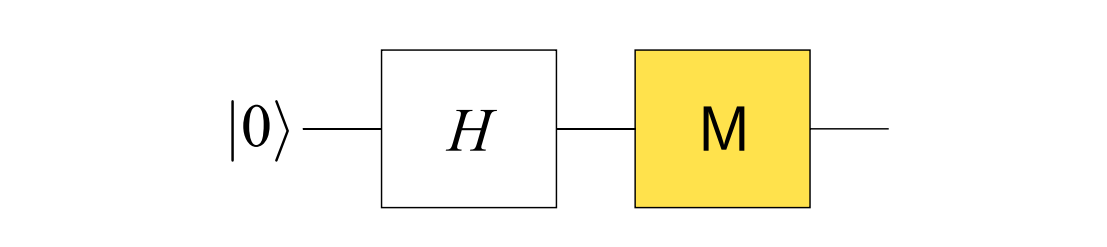
\includegraphics[width=0.7\linewidth]{img/MuenzwurfSchaltkreis.png}
    \caption{Schaltkreis für den Münzwurf Algorithmus}
    \label{fig:Muenzwurf}
\end{figure}


Schaltkreise eigenen sich dafür Quantenalgorithmen zu veranschaulichen. Auf diese wird später genauer eingegangen.\\

Zuerst wird ein Quantenbit in den Zustand $\left|0\right\rangle$ gebracht. Man könnte es auch in den Zustand $\left|1\right\rangle$ versetzen. Das macht für diesen Algorithmus keinen Unterschied. Danach wendet man die Hadamard-Transformation darauf an, um das Quantenbit in eine Superposition zu bringen, in der die Wahrscheinlichkeit $\left|0\right\rangle$ oder $\left|1\right\rangle$ zu messen gleich verteilt ist. Anschließend wird gemessen und die Superposition zerfällt zufällig in einen der Zustände $\left|0\right\rangle$ oder $\left|1\right\rangle$.

Formal beschrieben sieht der Algorithmus so aus:
\begin{align*}
    &\left|x\right\rangle \gets\ \left|0\right\rangle  \\
    &\left|x\right\rangle \gets\ H\left|x\right\rangle \\
    &Miss\left|x\right\rangle
\end{align*}

	
„$\left|x\right\rangle$“ ist dabei die Bezeichnung des Quantenbits auf dem gerechnet wird.

Mit diesem Algorithmus ist es möglich echte Zufallszahlen zu generieren, da es physikalisch unmöglich ist vorauszusagen, in welchen Zustand die Superposition zerfallen wird. Dies steht im Gegensatz zu einem echten Münzwurf, bei dem man das Wurfergebnis theoretisch berechnen könnte, wenn man sämtliche Variablen, wie z.B. Wurfhöhe, Drehmoment der Münze, Luftwiederstand, ect. kennen würde. Oder im Gegensatz zu einem herkömmlichen Computer, der nur Pseudozufallszahlen generieren kann. 
\subsection{Quantenregister}

Ein Quantenregister ist eine Aneinanderreihung mehrerer, voneinander unabhängiger Quantenbits. Diese werden benötigt, um Quantenschaltkreise zu realisieren, damit auf ihnen logische Operationen durchgeführt werden können. 

Der Zustand eines Quantenregisters der Länge m wird als m-faches Tensorprodukt aller Zustände der einzelnen Quantenbits des Registers dargestellt. Ein Quantenregister R mit 2 Qubits $\left|\left.x_0\right\rangle\right.$ und $\left|\left.x_1\right\rangle\right.$ in beispielsweise den Basiszuständen $\left|\left.x_0\right\rangle\right.=\binom{0}{1}$ und $\left|\left.x_1\right\rangle\right.=\binom{1}{0}$ befindet sich im Zustand:
\begin{equation}
    R=\left|\left.x_0\right\rangle\right.\otimes\left|\left.x_1\right\rangle\right.=\binom{0}{1}\otimes\binom{1}{0}=\left(\begin{matrix}0\\\begin{matrix}0\\\begin{matrix}1\\0\\\end{matrix}\\\end{matrix}\\\end{matrix}\right)
\end{equation}

Alternativ würde man $R=\left|1\right\rangle\otimes\left|0\right\rangle=\left|10\right\rangle$ schreiben. Manchmal werden die Basiszustände zur Übersichtlichkeit auch in Dezimalform dargestellt. $\left|10\right\rangle$ wäre demnach $\left|2\right\rangle$. \\

Wie auch die einzelnen Qubits, kann sich das gesamte Quantenregister in einer Superposition befinden. Sind die Qubits aus dem obigen Beispiel in den Zuständen 
$\left|\left.x_0\right\rangle\right.=\beta_0\left|\left.0\right\rangle\right.+\beta_1\left|\left.1\right\rangle\right.$ und $\left.\left|\left.x_1\right\rangle\right.=\gamma_0\left|\left.0\right\rangle\right.+\gamma_1\left|\left.1\right\rangle\right.\right.$
ist der Zustand des Quantenregisters 
\begin{equation}
\begin{aligned}
    R&=\left|\left.x_0\right\rangle\right.\left|\left.x_1\right\rangle\right.=\left(\beta_0\left|\left.0\right\rangle\right.+\beta_1\left|\left.1\right\rangle\right.\right)\cdot(\gamma_0\left|\left.0\right\rangle\right.+\gamma_1\left|\left.1\right\rangle\right.)\\
    &=\beta_0\gamma_0\left.\left|0\right\rangle\left|0\right\rangle\right.+\beta_0\gamma_1\left|\left.0\right\rangle\left|\left.1\right\rangle\right.\right.+\beta_1\gamma_0\left|\left.1\right\rangle\right.\left|\left.0\right\rangle\right.+\beta_1\gamma_1\left|\left.1\right\rangle\right.\left|\left.1\right\rangle\right.
\end{aligned}
\end{equation}
Substituiert man $\beta_i\gamma_j=\alpha_{ij}$, ergibt sich der Zustand
\begin{equation}
    R=\alpha_{00}\left|\left.0\right\rangle\right.\left|\left.0\right\rangle\right.+\alpha_{01}\left|\left.0\right\rangle\left|\left.1\right\rangle\right.\right.+\alpha_{10}\left|\left.1\right\rangle\right.\left|\left.0\right\rangle\right.+\alpha_{11}\left|\left.1\right\rangle\right.\left|\left.1\right\rangle\right.
\end{equation}
Und kann als
\begin{equation}
    R=\alpha_{00}\left|\left.00\right\rangle\right.+\alpha_{01}\left|\left.01\right\rangle\right.+\alpha_{10}\left|\left.10\right\rangle\right.+\alpha_{11}\left|\left.11\right\rangle\right.
\end{equation}
Oder
\begin{equation}
    R=\alpha_0\left|\left.0\right\rangle\right.+\alpha_1\left|\left.1\right\rangle\right.+\alpha_2\left|\left.2\right\rangle\right.+\alpha_3\left|\left.3\right\rangle\right.
\end{equation}
geschrieben werden.\\

Da aus $\left|\beta_0\right|^2+\left|\beta_1\right|^2=1$ und $\left|\gamma_0\right|^2+\left|\gamma_1\right|^2=1$ sich $\left|\alpha_{00}\right|^2+\left|\alpha_{01}\right|^2+\left|\alpha_{10}\right|^2+\left|\alpha_{11}\right|^2=$1 ergibt, bildet $\alpha$ die Amplitude für den jeweiligen Zustand $\left|\left.00\right\rangle\right.$, $\left|\left.01\right\rangle\right.$, $\left|\left.10\right\rangle\right.$ und $\left|\left.11\right\rangle\right.$. \\

Allgemeiner gefasst befindet sich ein Quantenregister R der Länge n im Zustand 
\begin{equation}
    R=\sum_{i=0}^{2^n-1}{\alpha_i\left|\left.i\right\rangle\right.},
\end{equation}
für den die Bedingung
\begin{equation}
    \sum_{i=0}^{2^n-1}\left|\alpha_i\right|^2=1
\end{equation}
gilt. Dabei entspricht $i=0,...,2^n-1$ der Dezimaldarstellung der Bits im Quantenregister und $\left|\alpha_i\right|^2$ der Wahrscheinlichkeit, dass sich das Register nach einer Messung im jeweiligen Zustand $\left|\left.i\right\rangle\right.$ befindet.\\

Es ist möglich Transformationen nicht nur auf einzelnen Quantenbits durchzuführen, sondern auch auf ganze Register. Um eine Transformation auf einem Register durchzuführen, muss zuerst ein n-faches Tensorprodukt der Transformationsmatrix mit sich selbst berechnet werden. n ist dabei die Länge des Registers. Da ein Tensorprodukt nur zwischen Matrizen derselben Größe berechnet werden kann, ist es nur möglich Transformationen auf $2^n$ langen Registern durchzuführen. \\

Die Transformationen $A_1,\ldots,A_{2^n}$ auf die Qubits $\left|\left.x_1\right\rangle\right.$, $\ldots,\left|\left.x_{2^n}\right\rangle\right.$ mit jeweils $A_i$ auf $\left|\left.x_i\right\rangle\right.$ entsprechen also der Transformation $A_1\otimes,\ldots,\otimes A_{2^n}$ auf das Register $\left|\left.x_1,\ldots,x_{2^n}\right\rangle\right.$.

Möchte man die Hadamard-Transformation H auf ein Register $R=\left|00\right\rangle$ anwenden, müsste man zuerst die Hadamard-Transformation auf Registerebene 
\begin{equation}
    H\otimes H\ =\ H_2=\ \frac{1}{\sqrt2}\left(\begin{matrix}H&H\\H&-H\\\end{matrix}\right)=\frac{1}{2}\left(\begin{matrix}\begin{matrix}1&1\\1&-1\\\end{matrix}&\begin{matrix}1&1\\1&-1\\\end{matrix}\\\begin{matrix}1&1\\1&-1\\\end{matrix}&\begin{matrix}-1&-1\\-1&1\\\end{matrix}\\\end{matrix}\right)
\end{equation}
bilden. Daraus ergibt sich
\begin{equation}
    H_2R\ =\frac{1}{2}\left(\begin{matrix}\begin{matrix}1&1\\1&-1\\\end{matrix}&\begin{matrix}1&1\\1&-1\\\end{matrix}\\\begin{matrix}1&1\\1&-1\\\end{matrix}&\begin{matrix}-1&-1\\-1&1\\\end{matrix}\\\end{matrix}\right)\left(\begin{matrix}1\\\begin{matrix}0\\\begin{matrix}0\\0\\\end{matrix}\\\end{matrix}\\\end{matrix}\right)=\left(\begin{matrix}\frac{1}{2}\\\frac{1}{2}\\\frac{1}{2}\\\frac{1}{2}\\\end{matrix}\right)\verb|,|
\end{equation}
beziehungsweise 
\begin{equation}
    \frac{1}{2}\left(\left|\left.00\right\rangle\right.+\left|\left.01\right\rangle\right.+\left|\left.10\right\rangle\right.+\left|\left.11\right\rangle\right.\right)
\end{equation}
    oder
\begin{equation}
    \frac{1}{2}\left(\left|\left.0\right\rangle\right.+\left|\left.1\right\rangle\right.+\left|\left.2\right\rangle\right.+\left|\left.3\right\rangle\right.\right).
\end{equation}
Dabei bleibt die Bedingung 
\begin{equation}
    \sum_{i=0}^{2^n-1}\left|\alpha_i\right|^2=1
\end{equation}
 Mit n = 2 und $\alpha_i=\frac{1}{2}\forall i$ erfüllt. Die Wahrscheinlichkeit, dass jeder Basiszustand nach der Messung auftritt, ist gleichverteilt. Diese Berechnung kann genutzt werden, um echte Zufallszahlen zwischen 0 und 3 zu generieren. Formal beschrieben sieht der Algorithmus aus, wie folgt:
 \begin{align*}
     &R=\left|\left.x_1x_0\right\rangle\right.\gets\left|\left.00\right\rangle\right.\\
	&R=H_2R\\
	&Miss R
 \end{align*}

Dieser Algorithmus kann auf eine beliebige Registergröße $2^n$ erweitert werden. 
Allerdings ist das Rechnen auf Registerebene bisher nur mathematisch sinnvoll. Tatsächlich werden sämtliche Rechenschritte in lokalen unitären Transformationen durchgeführt. „Lokal“ heißt in diesem Fall, dass maximal drei Qubits an der Berechnung beteiligt sind, da es physikalisch einfacher ist Transformationen auf drei Qubits auszuführen als auf $2^n$ mit beliebig hohen n. Zudem sind mindestens drei Qubit notwendig, um klassische Rechenverfahren in Quantenalgorithmen zu überführen. Dies wird später aufgegriffen.\\

In den beiden Münzwurfbeispielen wurde die Hadamard-Transformation nur auf Quantenbits oder -register angewendet, bei denen sich alle Bits im Zustand $\left|0\right\rangle$ befunden haben. Ein n langes Quantenregister R, dessen Bits sich alle im Zustand $\left|0\right\rangle$ befunden haben und auf das die Hadamard-Transformation angewandt wurde, kann wie folgt dargestellt werden:
\begin{equation}
    R=\frac{1}{\sqrt{2^n}}\sum_{i=0}^{2^n-1}\left|\left.i\right\rangle\right.
\end{equation}
Diese Darstellung reicht allerdings nicht aus, um Quantenregister abzubilden, dessen Quantenbits sich vor der Hadamard-Transformation teilweise im Zustand $\left|1\right\rangle$ befunden haben. Wendet man die Hadamard-Transformation auf ein Register $\left|xy\right\rangle$ an, das sich im Zustand $\left|01\right\rangle$ befindet, sähe das Quantenregister vor dem Ausmultiplizieren wie folgt aus:
\begin{equation}
    \left|\left.01\right\rangle\right.{\buildrel H_2\over\longrightarrow}\frac{1}{\sqrt2}(\left|\left.0\right\rangle\right.+\left|\left.1\right\rangle\right.)\cdot\frac{1}{\sqrt2}(\left|\left.0\right\rangle\right.-\left|\left.1\right\rangle\right.).
\end{equation}
Man kann an dieser Stelle die Information, ob sich die jeweiligen Quantenbits vorher im Zustand $\left|0\right\rangle$ oder $\left|1\right\rangle$ befunden haben, in das Vorzeichen ziehen:
\begin{equation}
    \left|\left.xy\right\rangle\right.{\buildrel H_2\over\longrightarrow}\frac{1}{\sqrt2}(\left|\left.0\right\rangle\right.+{(-1)}^x\left|\left.1\right\rangle\right.)\cdot\frac{1}{\sqrt2}(\left|\left.0\right\rangle\right.+{(-1)}^y\left|\left.1\right\rangle\right.).
\end{equation}
Ausmultipliziert ergibt dies: 
\begin{equation}
    \frac{1}{2}\left(\left|\left.00\right\rangle\right.+\left(-1\right)^x\left|\left.01\right\rangle\right.+\left(-1\right)^y\left|\left.10\right\rangle\right.+\left(-1\right)^{x\oplus y}\left|\left.11\right\rangle\right.\right).
\end{equation}
Allgemeiner gefasst:
\begin{equation}
    \frac{1}{2}\left(\left(-1\right)^{\left(0,0\right)\oplus z}\left|\left.00\right\rangle\right.+\left(-1\right)^{\left(0,1\right)\oplus z}\left|\left.01\right\rangle\right.+\left(-1\right)^{\left(1,0\right)\oplus z}\left|\left.10\right\rangle\right.+\left(-1\right)^{\left(1,1\right)\oplus z}\left|\left.11\right\rangle\right.\right.),
\end{equation}
mit $z={(x,y)}^T$.

Anhand der letzten Darstellung kann man ein Quantenregister der Länge n im Zustand
$x\in{\{0,1\}}^n$, auf das die Hadamard-Transformation angewandt wurde, wie folgt darstellen:
\begin{equation}
    H_n\left|\left.x\right\rangle\right.=\frac{1}{\sqrt{2^n}}\sum_{y\in{0,1}^n}\left(-1\right)^{x\cdot y}\left|\left.y\right\rangle\right..
\end{equation}
Dabei ist $x\cdot y$ das Skalarprodukt $\oplus_{i=1}^nx_iy_i$ der Vektoren $x,y\in{\{0,1\}}^n$. \\
Auch die Hadamard-Transformation ist reversibel. Nehmen wir das vorherige Beispiel:
\begin{equation}
    \left|\left.01\right\rangle\right.{\buildrel H_2\over\longrightarrow}\frac{1}{\sqrt2}(\left|\left.0\right\rangle\right.+\left|\left.1\right\rangle\right.)\cdot\frac{1}{\sqrt2}(\left|\left.0\right\rangle\right.-\left|\left.1\right\rangle\right.).
\end{equation}
Wendet man die Hadamard-Transformation erneut an, ergibt sich:
\begin{equation}
    \begin{aligned}
    &\frac{1}{\sqrt2}\left(\left|\left.0\right\rangle\right.+\left|\left.1\right\rangle\right.\right)\cdot\frac{1}{\sqrt2}\left(\left|\left.0\right\rangle\right.-\left|\left.1\right\rangle\right.\right)\\
    &{\buildrel H_2\over\longrightarrow}\frac{1}{\sqrt2}\left(\frac{1}{\sqrt2}\left(\left|\left.0\right\rangle\right.+\left|\left.1\right\rangle\right.\right)+\frac{1}{\sqrt2}\left(\left|\left.0\right\rangle\right.-\left|\left.1\right\rangle\right.\right)\right)\cdot\frac{1}{\sqrt2}\left(\frac{1}{\sqrt2}\left(\left|\left.0\right\rangle\right.+\left|\left.1\right\rangle\right.\right)-\frac{1}{\sqrt2}\left(\left|\left.0\right\rangle\right.-\left|\left.1\right\rangle\right.\right)\right)\\
    &=\frac{1}{\sqrt2}\left(\frac{1}{\sqrt2}\left(\left|\left.0\right\rangle\right.+\left|\left.0\right\rangle\right.\right)\right)\cdot\frac{1}{\sqrt2}\left(\frac{1}{\sqrt2}\left(\left|\left.1\right\rangle\right.+\left|\left.1\right\rangle\right.\right)\right)\\
    &=\frac{1}{2}\left(\left|\left.0\right\rangle\right.+\left|\left.0\right\rangle\right.\right)\cdot\frac{1}{2}\left(\left|\left.1\right\rangle\right.+\left|\left.1\right\rangle\right.\right)\ =\frac{1}{4}\left(\left|\left.01\right\rangle\right.+\left|\left.01\right\rangle\right.+\left|\left.01\right\rangle\right.+\left|\left.01\right\rangle\right.\right)=\left|\left.01\right\rangle\right..
\end{aligned}
\end{equation}

Die Reversibilität der Hadamard-Transformation ist für komplexere Algorithmen von Bedeutung. Bevor auf diese und deren Darstellung in Form von Quantenschaltkreisen eingegangen werden kann, muss noch der Vorgang des Messens genauer beschrieben werden.
\subsection{Messen}

Die Messung „Miss$\left|x\right.\rangle$“ ist die einzige Transformation in der Quanteninformatik, die nicht reversibel, beziehungsweise unitär ist. Beim Messen verliert ein Quantenbit seine Superposition und fällt zufällig, je nach Wahrscheinlichkeitsverteilung, in einen der Basiszustände, in deren Kontext gemessen wurde. Aus diesen Zuständen ist nicht zu errechnen in welchem Zustand sich das Quantenbit vor der Messung befunden hat. \\
Bisher wurde davon ausgegangen, dass ein Quantenbit nur in die Zustände $\left|0\right.\rangle$ oder $\left|1\right.\rangle$ zerfallen kann. Dies geschieht allerdings nur dann, wenn $\left|0\right.\rangle$ und $\left|1\right.\rangle$ die Basis der Messung bilden. Genauer gesagt, wenn diese die Basis bilden, in deren Vektorraum der Zustand des Quantenbits abgebildet wird. 
In der Quanteninformatik müssen diese Basen die Eigenschaften der Orthonormalbasen erfüllen. Die Basis zur Abbildung eines Quantenbits $\{\left|0\right.\rangle,\left|1\right.\rangle\}$ erfüllt diese Voraussetzungen. Diese wird Standardbasis genannt. Die Basis zur Abbildung eines Registers mit zwei Quantenbits $\{\left|00\right.\rangle,\left|01\right.\rangle\left|10\right.\rangle,\left|10\right.\rangle\}$ erfüllt diese Bedingung ebenfalls. Diese wird schließlich aus dem einfachen Tensorprodukt der Standardbasis mit sich selbst gebildet. 
Misst man als Beispiel das Register mit zwei Quantenbits, zerfällt der Zustand des Registers in einen der zugehörigen Basiszustände und man erhält ein Messergebnis.
Mathematisch ausgedrückt bestimmen beim Messen des 2 Bit-Quantenregisters ``die Projektionen auf die eindimensionalen Unterräume 
$$Span\{\left|00\right.\rangle\},Span\{\left|01\right.\rangle\},Span\{\left|10\right.\rangle\}\ \text{und}\ Span\{\left|11\right.\rangle\}$$
das Ergebnis.''\ \footnote{\cite[S. 47]{homeister_quantum_2022}} \\
Diese oben genannte Folge von Unterräumen, die aus der disjunkten Zerlegung der Orthonormalbasis: $\{\left|00\right.\rangle,\left|01\right.\rangle,\left|10\right.\rangle,\left|11\right.\rangle\}$, entstehen, nennt man ``Observable''.
Diese Unterräume enthalten jeweils einen Basisvektor, der jeweils einen der Zustände bildet, der nach dem vollständigen Messen des Registers $\textit{beobachtet}$ werden kann.\\

Zwei zusätzliche Dinge sind beim Messen möglich. Man kann zum einen nur einzelne Bits messen, statt des gesamten Registers. Zum anderen kann man zum Messen eine andere Basis verwenden, als zum Projektieren des Zustandes in einen Vektorraum verwendet wird. 

Das Messen einzelner Bits in einem Register ist in manchen Algorithmen wichtig, um anhand eines Zwischenergebnisses zu bestimmen, welche Folgetransformationen durchgeführt werden müssen. Quantenteleportation ist ein Beispiel dafür. Auch dazu später mehr.\\

Misst man in einem Register mit zwei Bits im Zustand $\left|\phi\right.\rangle$ beispielsweise nur das erste Bit, bestimmen die Projektionen 
$$Span\{\left|00\right.\rangle\,\left|01\right.\rangle\} \text{ und }Span\{\left|10\right.\rangle\,\left|11\right.\rangle\}$$ das Ergebnis.
In dem Fall geht das Register ``mit der Wahrscheinlichkeit
$$\left|\alpha_{00}\right|^2+\left|\alpha_{01}\right|^2$$
in den Zustand 
$$\left|\phi'\right.\rangle=\frac{\alpha_{00}\left|00\right.\rangle+\alpha_{01}\left|01\right.\rangle}{\sqrt{\left|\alpha_{00}\right|^2+\left|\alpha_{01}\right|^2}}$$
über und mit Wahrscheinlichkeit
$$\left|\alpha_{10}\right|^2+\left|\alpha_{11}\right|^2$$
in den Zustand 
$$\left|\phi'\right.\rangle=\frac{\alpha_{10}\left|00\right.\rangle+\alpha_{11}\left|01\right.\rangle}{\sqrt{\left|\alpha_{10}\right|^2+\left|\alpha_{11}\right|^2}}.$$
Wir erfahren bei der Messung nur den Wert des gemessenen Bits, nicht
die Amplituden des Folgezustandes.''\ \footnote{\cite[S. 47]{homeister_quantum_2022}}\\

Das Messen in einer anderen Basis, als der, die zur Projektion ein einen Vektorraum genutzt wird, kann genutzt werden, um die Superposition des Quantenbits nach der Messung nicht vollständig zu zerstören. 
Misst man ein Quantenbit in der Basis $\{\left|+\right.\rangle,\left|-\right.\rangle\}$ mit $\left|+\right.\rangle=\frac{1}{\sqrt{2}}\left(\left|0\right.\rangle+\left|1\right.\rangle\right)$ und $\left|-\right.\rangle=\frac{1}{\sqrt{2}}\left(\left|0\right.\rangle-\left|1\right.\rangle\right)$ erhält man als Ergebnis entweder den Zustand $\frac{1}{\sqrt{2}}\left(\left|0\right.\rangle+\left|1\right.\rangle\right)$ oder $\frac{1}{\sqrt{2}}\left(\left|0\right.\rangle-\left|1\right.\rangle\right)$. Dies ist immer noch eine Superposition. Daher kann nach der Messung mit dem Quantenbit noch weiter gerechnet werden. Allerdings ist es auch hierbei nicht möglich den Zustand zu ermitteln, in dem sich das Bit vor der Messung befunden hat. Die Messung bleibt irreversibel. Die Basis $\{\left|+\right.\rangle,\left|-\right.\rangle\}$ wird ``Hadamard-Basis'' genannt.\\\newpage

Zur Veranschaulichung kann die folgende Abbildung dienen\footnote{\cite[S. 44]{homeister_quantum_2022}}: \\


\begin{figure}[!h]
    \centering
    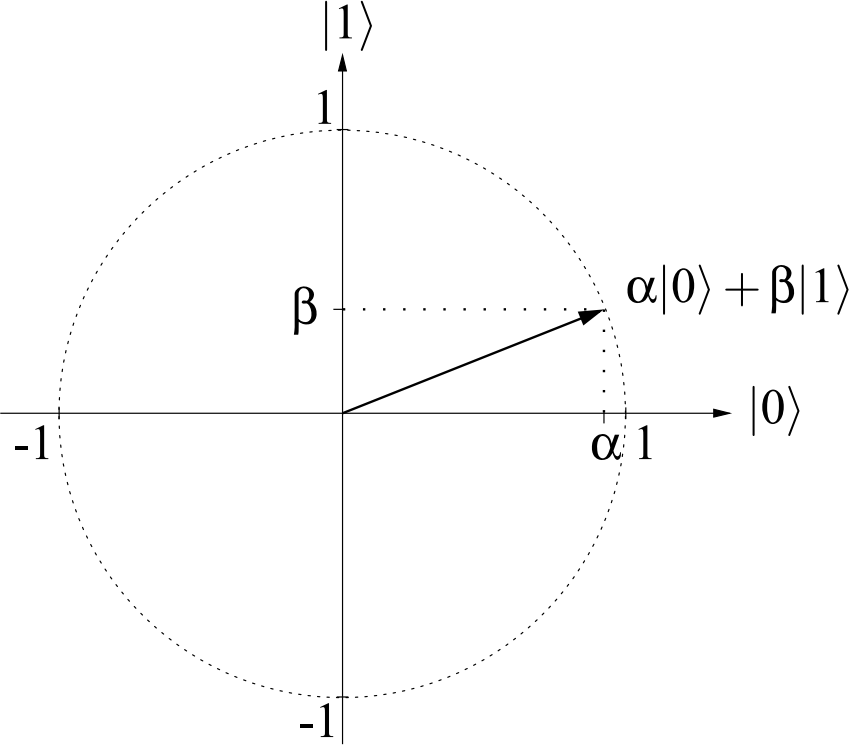
\includegraphics[width=0.5\linewidth]{img/Zustandsvektor_Standardbasis.png}
    \caption{Zustandsvektor in der Standardbasis}
    \label{fig:Standardbasis}
\end{figure}

Es wird ein Zustandsvektor in der Standardbasis dargestellt. Die Länge der Projektionen des Zustandsvektors auf den beiden Achsen bestimmen die Wahrscheinlichkeit, mit der, nach der Messung, einer der Zustände eingenommen wird. Mit der Wahrscheinlichkeit $\left|\alpha\right|^2$ wird der Zustand nach der Messung $\left|0\right.\rangle$ sein und mit der Wahrscheinlichkeit $\left|\beta\right|^2$ $\left|1\right.\rangle$. 

In der folgenden Abbildung wird derselbe Zustandsvektor gezeigt, mit dem Unterschied, dass die Koordinatenachsen nach der Hadamard-Basis ausgerichtet sind\footnote{\cite[S. 45]{homeister_quantum_2022}}.

\begin{figure}[h]
    \centering
    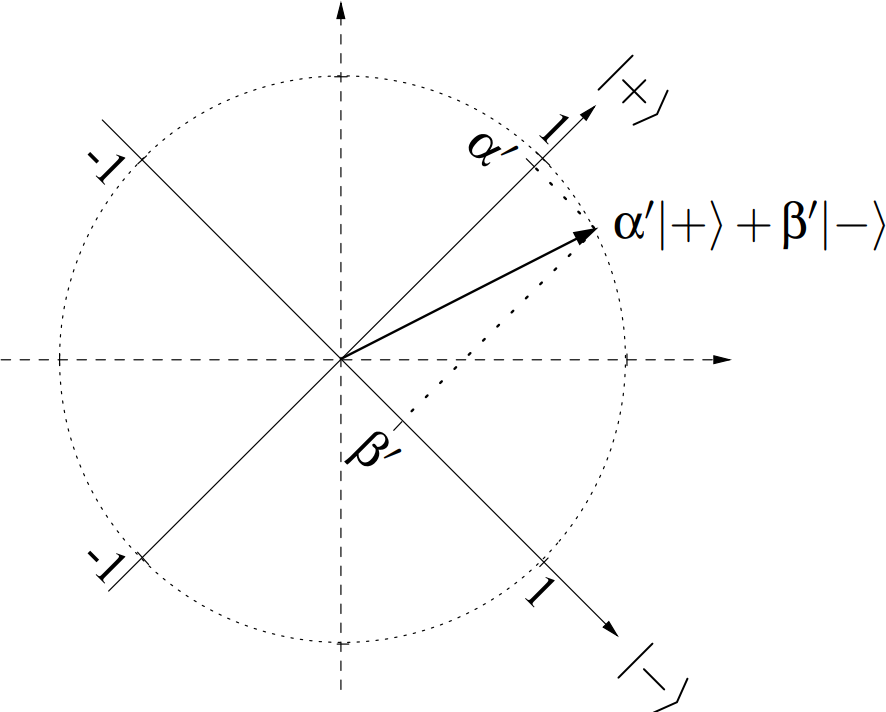
\includegraphics[width=0.5\linewidth]{img/Zustandsvektor_Hadamard-Basis.png}
    \caption{Zustandsvektor in der Hadamard-Basis}
    \label{fig:Hadamardbasis}
\end{figure}

Die Projektionen der Achsen haben sich im Vergleich zur Projektion auf die Standardbasis verändert. Mit der Wahrscheinlichkeit $\left|\alpha'\right|^2$ wird nach dem Messen der Zustand $\left|+\right.\rangle$ angenommen und mit der Wahrscheinlichkeit $\left|\beta'\right|^2$ $\left|-\right.\rangle$. 

Mathematisch sieht diese ``Basistransformation'' aus wie folgt:
\begin{equation}
    \alpha\left|0\right.\rangle+\beta\left|1\right.\rangle=\alpha'\frac{1}{\sqrt{2}}\left(\left|0\right.\rangle+\left|1\right.\rangle\right)+\beta'\frac{1}{\sqrt{2}}\left(\left|0\right.\rangle-\left|1\right.\rangle\right).
\end{equation}


Allgemeiner lässt sich zusammenfassen: ``Register R bestehe aus n Quantenbits und befinde sich im Zustand
$$\left|\phi\right.\rangle=\sum_{i=0}^{2^n-1}\alpha_i\left|i\right.\rangle$$
Wir messen bezüglich der Basis
$\left|0'\right.\rangle,\left|1'\right.\rangle,...,\left|(2^n-1)'\right.\rangle$
aus zueinander orthogonalen Vektoren der Länge 1.''\ \footnote{\cite[S. 46]{homeister_quantum_2022}} Dies ist eine andere Basis, als die in der sich $\left|\phi\right.\rangle$ befindet. ``Dabei wird die Superposition von $\left|\phi\right.\rangle$ zerstört. Hat $\left|\phi\right.\rangle$ bezüglich der Messbasis die Darstellung
$$\sum_{i=0}^{2^n-1}\alpha'_i\left|i\right.\rangle\verb|,|$$
so finden wir das Register nach der Messung mit Wahrscheinlichkeit $\left|\alpha'_i\right|^2$ im Zustand $\left|i'\right.\rangle$ vor.  Sämtliche anderen Informationen gehen dabei
verloren.''\ \footnote{\cite[S. 46]{homeister_quantum_2022}}\\

Das Messen einzelner Bits oder ganzer Register, sowie das Messen von Teilen eines Registers in der Standardbasis oder auch in einer anderen umfasst alles, was beim Messen möglich ist.

